%----------------------------------------------------------------------
% COMPUTATIONAL PHYSICS - PROJECT 3
% ENERGY SPECTRUM OF QUANTUM SPIN CHAINS
%----------------------------------------------------------------------

\documentclass[a4paper]{IEEEtran} 
\usepackage{amssymb}
\usepackage{moreverb}
\usepackage[cmex10]{amsmath} 
\usepackage{cite} 
\usepackage{graphicx} 
\usepackage[colorlinks=false, hidelinks]{hyperref} 

\usepackage{listings} 
\usepackage{color} 
\usepackage{xcolor}  
\usepackage{microtype} 
\usepackage{microtype} 
\usepackage{inconsolata} 
\usepackage[framemethod=TikZ]{mdframed} 
\usepackage{alltt}
\usepackage{sverb} 
\usepackage{verbatim} 
\usepackage{pifont} 
\usepackage{alltt} 
\usepackage{helvet} 

%----------------------------------------------------------------------
% CODE LISTING SETTINGS
%----------------------------------------------------------------------

\lstset{language=fortran,
        %basicstyle=\footnotesize\ttfamily, 
        basicstyle=\small\ttfamily,
        columns=fullflexible, 
        %title=\lstname, 
        numbers=left, stringstyle=\texttt, 
        numberstyle={\tiny\texttt}, 
        keywordstyle=\color{blue}, 
        commentstyle=\color{darkgreen}, 
        stringstyle=\color{purple} } 


\mdfsetup{skipabove=\topskip, skipbelow=\topskip} 

\definecolor{codebg}{rgb}{0.99,0.99,0.99}

\global\mdfdefinestyle{code}{%
    frametitlerule=true,%
    frametitlefont=\small\bfseries\ttfamily,%
    frametitlebackgroundcolor=lightgray,%
    backgroundcolor=codebg,%
    linecolor=gray, linewidth=0.5pt,%
    leftmargin=0.5cm, rightmargin=0.5cm,%
    roundcorner=2pt,%
    innerleftmargin=5pt
}

\global\mdfdefinestyle{code2}{%
    topline=false,%
    bottomline=false,%
    leftline=true,%
    rightline=false,%
    backgroundcolor=codebg,%
    linecolor=gray, linewidth=0.5pt,%
    leftmargin=0.0cm, rightmargin=0.0cm,%
    innerleftmargin=1pt
}

\newcommand{\showcode}[1]{\begin{mdframed}[style=code] %
                            \lstinputlisting{#1}% 
                          \end{mdframed}% 
}

\newcommand{\showsmallcode}[1]{\begin{mdframed}[style=code2] %
        \lstinputlisting[basicstyle=\ttfamily\tiny]{#1}% 
                          \end{mdframed}% 
}




%----------------------------------------------------------------------
% IEEE SETTINGS
%----------------------------------------------------------------------

\interdisplaylinepenalty=2500
\setlength{\IEEEilabelindent}{\IEEEilabelindentB}

\markboth{630--364 Computational Physics}{} 

%----------------------------------------------------------------------
% TITLE
%----------------------------------------------------------------------

\title{Energy Spectrum of Quantum Spin Chains} 
\author{Michael Papasimeon\\ 10 September 1997} % \\
\date{10 September 1997}

%----------------------------------------------------------------------
% BEGIN DOCUMENT
%----------------------------------------------------------------------

\begin{document}
\maketitle

\section{Aims}
The main aims are to:
    \begin{itemize}
        \item Write a computer program which represents the complete set of states
              of a quantum spin chain of size $N$.
        \item Modify the program to compute the Hamiltonian matrix of the quantum spin chain
        \item Use package routines to tri-diagonalise and then to diagonalise the Hamiltonian
              matrix which will give us the eigenvalues of the matrix.
        \item The eigenvalues are the energy eigenstates of the quantum spin chain obtained
              from the Schrodinger equation $H|\Psi\rangle = E|\Psi\rangle$. This gives
              us the energy spectrum of the quantum spin chain for a given $N$.
        \item Investigate the energy spectrum of the quantum spin chain if it is placed
              in a magnetic field oriented along it's $z$-axis with a magnetic field
              strength of $B_z\mu$.
    \end{itemize}

\section{Background}
    The diagram below represents a quantum spin chain of $N$ particles.
    Each particle's $z$-component spin is either in a 
    spin up $\left(+\frac{1}{2}\right)$ state or
    a spin down $\left(-\frac{1}{2}\right)$ state.
    \begin{center}
        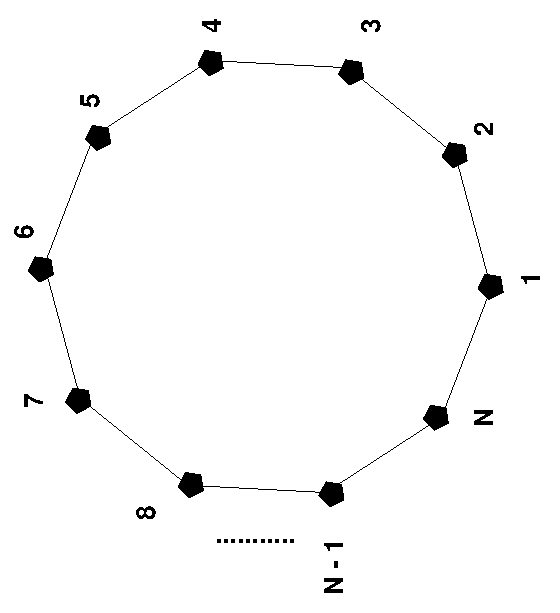
\includegraphics[angle=-90, width=4cm]{chain.eps}
    \end{center}
    Each particle interacts with it's neighbour. The interaction can be described
    with the Heisenberg Hamiltonian $H$,
        \[ H = \sum_{i = 1}^{N} \vec{S}(i) \cdot \vec{S}(i+1) \]
    where $i$ is the particle site, and $\vec{S}(i)$ is a vector of spin
    operators at site $i$, such that
        $\vec{S}(i) = (S_x(i), S_y(i), S_z(i) ) i$
    The chain can be in a number of different spin states at any one time. There
    are $2^N$ possible states for $N$ particles. The complete set of states 
    is given by:
        \[ \{| \phi_n \rangle \} = \{ | S_z(1)S_z(2)S_z(3).....S_z(N-1)S_z(N) \rangle \} \]
    For example for a chain with $N=2$, the complete set of states is given by:
        \[ \{|\phi_n\rangle\} = \{ |\uparrow \uparrow \rangle,
                                   |\uparrow \downarrow \rangle,
                                   |\downarrow \uparrow \rangle,
                                   |\downarrow \downarrow \rangle\}\]
    Using this information we can solve the Schrodinger eigenvalue equation of the
    system:
        \[ H|\psi\rangle = E|\psi\rangle\]
    This can be represented as a matrix equation:
        \[ Hx = E_n x\]
    where $E_n$ are the energy levels of the system, $x_n$ are the eigenvectors,
    and $H$ is the Heisenberg Hamiltonian matrix. Therefore:
        \[ x_n = \langle \phi_n | \psi \rangle \]
    and each matrix element $H_{nm}$ is given by:
        \[ H_{nm} = \langle \phi_n | H | \phi_m \rangle \]
    The Heisenberg Hamiltonian can be expanded as follows:
    \begin{eqnarray*}
    H & = & \sum_{i = 1}^{N} \vec{S}(i) \cdot \vec{S}(i+1) \\ 
    H & = & \sum_{i = 1}^{N} \left[ S_x(i)S_x(i+1) +
                                    S_y(i)S_y(i+1) +
                                    S_z(i)S_z(i+1) \right] \\
    \end{eqnarray*}
    Using the raising and lowering operators:
        \[ S_{\pm} = S_x(i) \pm iS_y(i) \]
    the Hamiltonian $H$ can be written in terms of two components such that:
        \[ H = \sum_{i=1}^{N} \left[ H_z(i) + H_f(i) \right] \]
    Where:
    \[ H_z(i) = S_z(i)S_z(i+1) \]
    \[ H_f(i) = \frac{1}{2} \left[ S_{+}(i)S_{-}(i+1) + S_{-}(i)S_{+}(i+1) \right]  \]


\section{Method}

    A Fortran program (\texttt{spin.f} in Appendix A)was written to represent the 
    complete set of states of a 
    quantum spin chain. The binary representation of 64-bit integers was used 
    to represent a possible state of a quantum spin chain. A given integer
    represents one possible state which the chain could be in. The binary representation
    of each integer is made up of 0's and 1's, where 0 represents spin down $-\frac{1}{2}$
    and 1 represents spin up $+\frac{1}{2}$. Each bit position represents the next site
    in the chain starting with the least significant bit as the first site.
    The table below shows the representation of the complete set of states using this method
    for a chain of size $N = 4$.

    \begin{table}
    \begin{center}
        \begin{tabular}{|c||c|c|c|c|} \hline
        State $|\phi_i\rangle$ & $2^3$ & $2^2$ & $2^1$ & $2^0$ \\ \hline \hline
        1 & 0 & 0 & 0 & 0 \\ \hline 
        2 & 0 & 0 & 0 & 1 \\ \hline
        3 & 0 & 0 & 1 & 0 \\ \hline
        4 & 0 & 0 & 1 & 1 \\ \hline
        5 & 0 & 1 & 0 & 0 \\ \hline
        6 & 0 & 1 & 0 & 1 \\ \hline
        7 & 0 & 1 & 1 & 0 \\ \hline
        8 & 0 & 1 & 1 & 1 \\ \hline
        9 & 1 & 0 & 0 & 0 \\ \hline
       10 & 1 & 0 & 0 & 1 \\ \hline
       11 & 1 & 0 & 1 & 0 \\ \hline
       12 & 1 & 0 & 1 & 1 \\ \hline
       13 & 1 & 1 & 0 & 0 \\ \hline
       14 & 1 & 1 & 0 & 1 \\ \hline
       15 & 1 & 1 & 1 & 0 \\ \hline
       16 & 1 & 1 & 1 & 1 \\ \hline
       \end{tabular}
       \vspace{1mm}
       \begin{center}
       Table 1 : Binary representation of complete set of states $\{|\phi_i\rangle\}$
       for $N=4$
       \end{center}
    \end{center}
    \end{table} 

    Once this is done functions to calculate the matrix elements $H_{mn}$ of the Hamiltonian
    matrix were written. Functions are needed to calculate the following quantaties:
    \begin{itemize}
        \item $\langle\phi_j|H_z|\phi_i\rangle$
        \item $\langle\phi_j|H_f|\phi_i\rangle$
        \item For the second part the contribution to each matrix element from the
              magnetic field $\langle\phi_j|H_m|\phi_i\rangle$
    \end{itemize}
    Once the Hamiltonian matrix for the particular spin chain has been calculated,
    package Fortran subroutines are used to tri-diagonalise and then diagonalise 
    the matrix. The elements along the diagonal of the resulting matrix give the
    energy eigenvalues of the system.

\section{Results}

    \subsection*{Energy Eigenvalues for Various Chain Sizes} 
    The table below shows the results of running the program for values of ranging
    from $N=2$ to $N=10$. The results in the table are $E_i/N$ where $i$ is the
    $i$th energy eigenstate and $N$ is the size of the quantum spin chain.

    \begin{table*}[ht] 
    \begin{center} 
        \begin{tabular}{|c|r|r|r|r|r|r|r|r|r|r|} \hline 
      $i$ & N=2   & N=3    & N=4    & N=5    & N=6    & N=7    & N=8       & N=9   & N=10\\ \hline  \hline
        0 & -0.75 & -0.583 & -1.140 & -1.534 & -2.754 & -4.411 & 1.860E-18 & 0.028 & -0.050 \\ \hline
        1 &  0.25 & -0.583 & -0.500 & -1.534 & -2.044 & -4.411 & 1.315E-17 & 0.028 & -0.050 \\ \hline
        2 &       & -0.083 & -0.500 & -0.531 & -2.044 & -2.811 & 2.862E-17 & 0.028 & -0.050 \\ \hline
        3 &       &        & -0.161 & -0.531 & -0.634 & -2.811 & 8.822E-18 & 0.028 & -0.050 \\ \hline
        4 &       &        &        & -0.150 & -0.634 & -0.823 & 1.713E-18 & 0.028 & -0.050 \\ \hline
        5 &       &        &        &        & -0.231 & -0.823 & -1.02E-17 & 0.028 & -0.050 \\ \hline
        6 &       &        &        &        &        & -0.179 & -3.65E-19 & 0.028 & -0.050 \\ \hline
        7 &       &        &        &        &        &        & -1.58E-19 & 0.028 & -0.050 \\ \hline
        8 &       &        &        &        &        &        &           & 0.028 & -0.050 \\ \hline
        9 &       &        &        &        &        &        &           &       & -0.050 \\ \hline
        \end{tabular}
        \vspace{1mm}
        \begin{center}
        Table 2 : Energy eigenvalues $E_i/N$ for different sized quantum spin chains
        \end{center}
    \end{center}
    \end{table*} 

    The table below shows the error code \texttt{ierr} given from the 
    \texttt{imtql1} subroutine for the different values of $N$. The error code
    is 0 if no error occured and a positive integer if an error occured. The value
    is set $j$ if the $j$th eigenvalue has not being determined after 30 iterations.

    \begin{table} 
    \begin{center}
        \begin{tabular}{|c|c|} \hline
        $N$ & \texttt{ierr} \\ \hline \hline
        2 & 0 \\ \hline
        3 & 0 \\ \hline
        4 & 0 \\ \hline
        5 & 0 \\ \hline
        6 & 0 \\ \hline
        7 & 0 \\ \hline
        8 & 1 \\ \hline
        9 & 6 \\ \hline
       10 & 2 \\ \hline
        \end{tabular}
        \vspace{1mm}
        \begin{center}
            Table 3 : Error Codes when diagonalising matrices for different $N$
        \end{center}
    \end{center}
    \end{table} 
  
    \subsection*{Spin Chains in the presence of a Magnetic Field of strength $B_z\mu$}
    Tables 4--9 show the energy eigenvalues for a chain of $N=6$, for different 
    values of the magnetic field strength $B_z\mu$. Each table 4--9, is for 
    a particular energy level. For example table 4 shows the results for the
    lowest energy level $E_0$.

    \begin{table}
        \begin{center}
        \begin{tabular}{|c|c|} \hline
        $B_z\mu$ & $E_0$  \\ \hline \hline
        0    & -2.75391005 \\ \hline
        1    & -3.2783723     \\ \hline 
        2    & -6.83931233  \\ \hline 
        5    & -17.976674 \\ \hline 
        10   & -36.7141831\\ \hline 
        20   & -74.2665118\\ \hline 
        50   & -186.98981\\ \hline 
        100  & -374.884865\\ \hline 
        500  & -1878.08728\\ \hline 
        1000 & -3757.09559\\ \hline 
        \end{tabular}
        \vspace{1mm}
        \begin{center}
            Table 4 : Energy Levels $E_0$ for varying $B_z\mu$ ( \texttt{1.dat} )
        \end{center}
        \end{center}
    \end{table}

    \begin{table} 
        \begin{center}
        \begin{tabular}{|c|c|} \hline
        $B_z\mu$ & $E_1$  \\ \hline \hline
        0    & -2.04416367 \\ \hline
        1    & -2.56881924 \\ \hline
        2    & -2.53377674 \\ \hline
        5    & -5.17989513 \\ \hline
        10   & -10.8286411 \\ \hline
        20   & -22.1589593 \\ \hline
        50   & -56.1740549 \\ \hline
        100  & -112.873705 \\ \hline
        500  & -566.484799  \\ \hline
        1000 & -1133.50039 \\ \hline
        \end{tabular}
         \vspace{1mm}
        \begin{center}
            Table 5 : Energy Levels $E_1$ for varying $B_z\mu$ ( \texttt{2.dat} )
        \end{center}
        \end{center}
    \end{table} 

    \begin{table} 
         \begin{center}
        \begin{tabular}{|c|c|} \hline
        $B_z\mu$ & $E_2$ \\ \hline \hline
        0    & -2.04416367 \\ \hline
        1    & -1.92139214\\ \hline
        2    & -1.89004066 \\ \hline
        5    & -3.20982437 \\ \hline
        10   & -6.00296934 \\ \hline
        20   & -11.7495711\\ \hline
        50   & -29.062476 \\ \hline
        100  & -57.9371933  \\ \hline
        500  & -288.967431  \\ \hline
        1000 & -577.759148 \\ \hline
        \end{tabular}
         \vspace{1mm}
        \begin{center}
            Table 6 : Energy Levels $E_2$ for varying $B_z\mu$ ( \texttt{3.dat} )
        \end{center}
        \end{center}
    \end{table} 

    \begin{table} 
         \begin{center}
        \begin{tabular}{|c|c|}  \hline
        $B_z\mu$ & $E_4$  \\ \hline \hline
        0    & -.63379594 \\ \hline
        1    &  -1.70564112 \\ \hline
        2    &  -1.84952222\\ \hline
        5    &  -2.34410019 \\ \hline
        10   &  -4.1755527 \\ \hline
        20   &  -8.63991335 \\ \hline
        50   &  -22.0554154 \\ \hline
        100  &  -44.422037 \\ \hline
        500  &  -223.368376 \\ \hline
        1000 &  -447.052966 \\ \hline
        \end{tabular}
         \vspace{1mm}
        \begin{center}
            Table 7 : Energy Levels $E_3$ for varying $B_z\mu$ ( \texttt{4.dat} )
        \end{center}
        \end{center}
    \end{table} 

    \begin{table} 
         \begin{center}
        \begin{tabular}{|c|c|} \hline
        $B_z\mu$ & $E_4$ \\ \hline \hline
        0    &  -.63379594 \\ \hline
        1    &  -.752476436 \\ \hline
        2    &  -1.66090753 \\ \hline
        5    &  -1.95855966 \\ \hline
        10   &  -2.98392009\\ \hline
        20   &  -5.64385606 \\ \hline
        50   &  -13.7786674 \\ \hline
        100  &  -27.3685291 \\ \hline
        500  &  -136.135355 \\ \hline
        1000 &  -232.535479 \\ \hline
        \end{tabular}
         \vspace{1mm}
        \begin{center}
            Table 8 : Energy Levels $E_4$ for varying $B_z\mu$ ( \texttt{5.dat} )
        \end{center}
        \end{center}
    \end{table} 

    \begin{table} 
         \begin{center}
        \begin{tabular}{|c|c|} \hline
        $B_z\mu$ & $E_5$ \\ \hline \hline
        0     & -.230940787 \\ \hline
        1     & -.596153367 \\ \hline
        2     & -.883832797 \\ \hline
        5     & -1.84820487 \\ \hline
        10    & -2.29196661 \\ \hline
        20    & -4.59813971 \\ \hline
        50    & -11.5734487\\ \hline
        100   & -23.2022424 \\ \hline
        500   & -116.238876 \\ \hline
        1000  & -232.535479 \\ \hline
        \end{tabular}
         \vspace{1mm}
        \begin{center}
            Table 9 : Energy Levels $E_5$ for varying $B_z\mu$ ( \texttt{6.dat} )
        \end{center}
        \end{center}
    \end{table} 

    The data in tables 4--9 have been plotted in the figure below. The lines
    \texttt{1.dat} -- \texttt{6.dat} correspond to the data in the different
    tables. Each lines in the plot corresponds to one of the six energy eigenvalues
    of the $N=6$ quantum spin chain.

    \begin{figure}[ht!]  
        \centering
        \caption{Plot 1 : Magnetic Field Strength $(B_z\mu)$ along the $x$-axis
             and Energy Level along the $y$-axis.}
        \label{fig:magnetic} 
        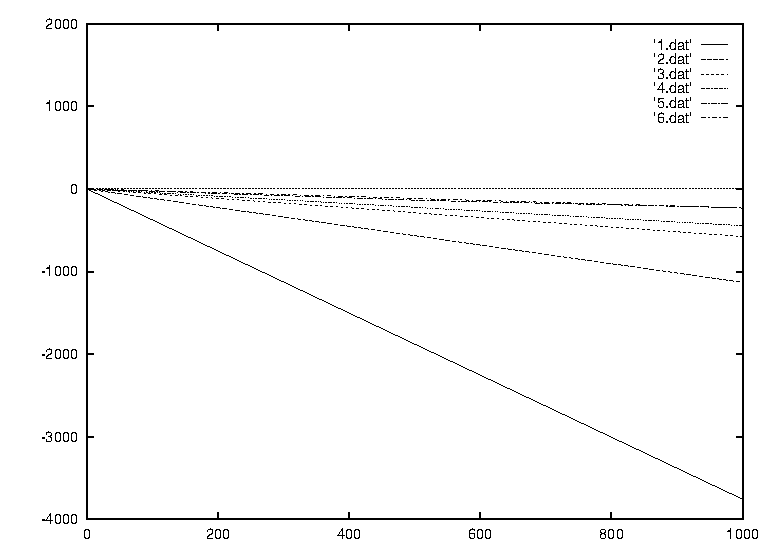
\includegraphics[width=\columnwidth]{magnetic.eps}
    \end{figure} 

\section{Discussion}

    Given the fact that there were some errors in the diagonalisation procedure
    as shown by Table 3 for $N=8,9,10$, the results shown in Table 2 for
    the energy levels of spin chains of this size are unlikely to 
    be correct. 

    This leaves us with energy levels for spin chains of size $N=2$ to
    $N=7$. For the ground state energy we expect the following result
    for $N \rightarrow \infty$:
        \[ \frac{E_0}{N} = -\ln(2) + \frac{1}{4} \simeq -0.443 \]
    This does not compare favourably with the results in Table 2, because
    as $N$ is increased $E_0/N$ is getting smaller with $E_0/7 = -4.411$.

    For $N=4$, the expected eigenvalues are:
    \begin{eqnarray*}
        \frac{E_0}{N} & = & -0.5  \\
        \frac{E_1}{N} & = & -0.25 \\
        \frac{E_2}{N} & = & -0.25 \\
        \frac{E_3}{N} & = & -0.25 \\
    \end{eqnarray*}
    Comparing to table 2, we see that the eigenvalue of -0.5 is the only one in agreement.
    The lack of agreement indicates an error in the program. However for the simple
    case of $N = 2$, the Hamiltonian matrix produced by the program for the 
    set of states described in table 1 is as follows:
    \[ H_{N=2} = \left( \begin{array}{rrrr}
    -0.5  &1  & 0  & 0 \\
    1  &-0.5  & 0  & 0 \\
    0  & 0  & 0.5  & 0 \\
    0  & 0  & 0  & 0.5 
    \end{array} \right) \]
    This result is as expected, which suggests that the routines \texttt{tred1}
    and/or \texttt{imtql1} may not be working as expected. However, due to 
    time considerations, the problem was not traced to any part of the code
    in particular.

    For the case when the quantum spin chain is in a magnetic field, we get
    the results shown in Plot 1. The plots follow the form of the expected
    output where:
        \[ E(\mu B_z) = -MB_z = -\mu B_z ( N(\uparrow) - N(\downarrow) ) \]
    The gradient of the plots is determined by the factor $( N(\uparrow) - N(\downarrow) ) $.
    For the six energy eigenvalues $( N(\uparrow) - N(\downarrow) ) > 0$. This indicates
    that for the $N=6$ spin chain, we have more particles in the spin up
    state than in the spin down state. The ground state energy has the largest
    gradient in Plot 1, indicating that there are more particles in the spin state
    than in the spin down state. This however decreases as the we go to higher
    energy states, making the gradient in the plot smaller.

% APPENDICES

\onecolumn

\appendix[Code Listing: spin.f] 
%\verbatimtabinput[6]{spin.f}
\showcode{spin.f} 

\end{document}
